\documentclass[a4paper, oneside]{memoir}
\usepackage[utf8]{inputenc}
\usepackage[T1]{fontenc}
\usepackage{pifont}
\usepackage{amssymb}
\usepackage{fourier}
\usepackage[dvipsnames]{xcolor}
\usepackage{tikz}
\usepackage{pdfpages}
\usepackage[sfdefault]{roboto}
\usepackage{color}

% Styles
\tikzstyle{teamshare} = [below, text width=5.4cm, inner sep = 0.5cm, text=white, align=center]
\tikzstyle{cardtext} = [below, text width=5.9cm, inner sep = 0.25cm, text centered]
\setlrmarginsandblock{0.9cm}{*}{1}
\setulmarginsandblock{1.49cm}{*}{1}
\checkandfixthelayout[nearest]
\pagestyle{empty}

% Define Commands
\newcommand{\condition}[1]{\textbf{#1}}
\newcommand{\character}[1]{\textbf{#1}}
\newdimen\titlespacing
\titlespacing=0.15cm

% Define Seperators
\newcommand{\seperator}[1]{\\ \vspace{\titlespacing} \hrulefill {} \tiny \bfseries #1 \normalfont \normalsize \hrulefill \\ \vspace{\titlespacing}}
\newcommand{\seperatoraction}{\seperator{POWER}}
\newcommand{\seperatordescription}{\seperator{DESCRIPTION}}
\newcommand{\seperatorcondition}{\seperator{CONDITION}}
\newcommand{\seperatorwin}{\seperator{HOW TO WIN}}
\newcommand{\redwinsection}{
	\seperatorwin
	You win if \character{Santa} does not gain the \condition{humbug} condition due to the \character{Grinch} stealing Christmas.
}
\newcommand{\greenwinsection}{
	\seperatorwin
	\small You win if \character{Santa} gains the \condition{humbug} condition due to the \character{Grinch} stealing Christmas.
}
\newcommand{\titlefrom}[1]{\\ \tiny > from #1 <\normalsize}

% Begin Document
\begin{document}
	
	% New Page
	\noindent 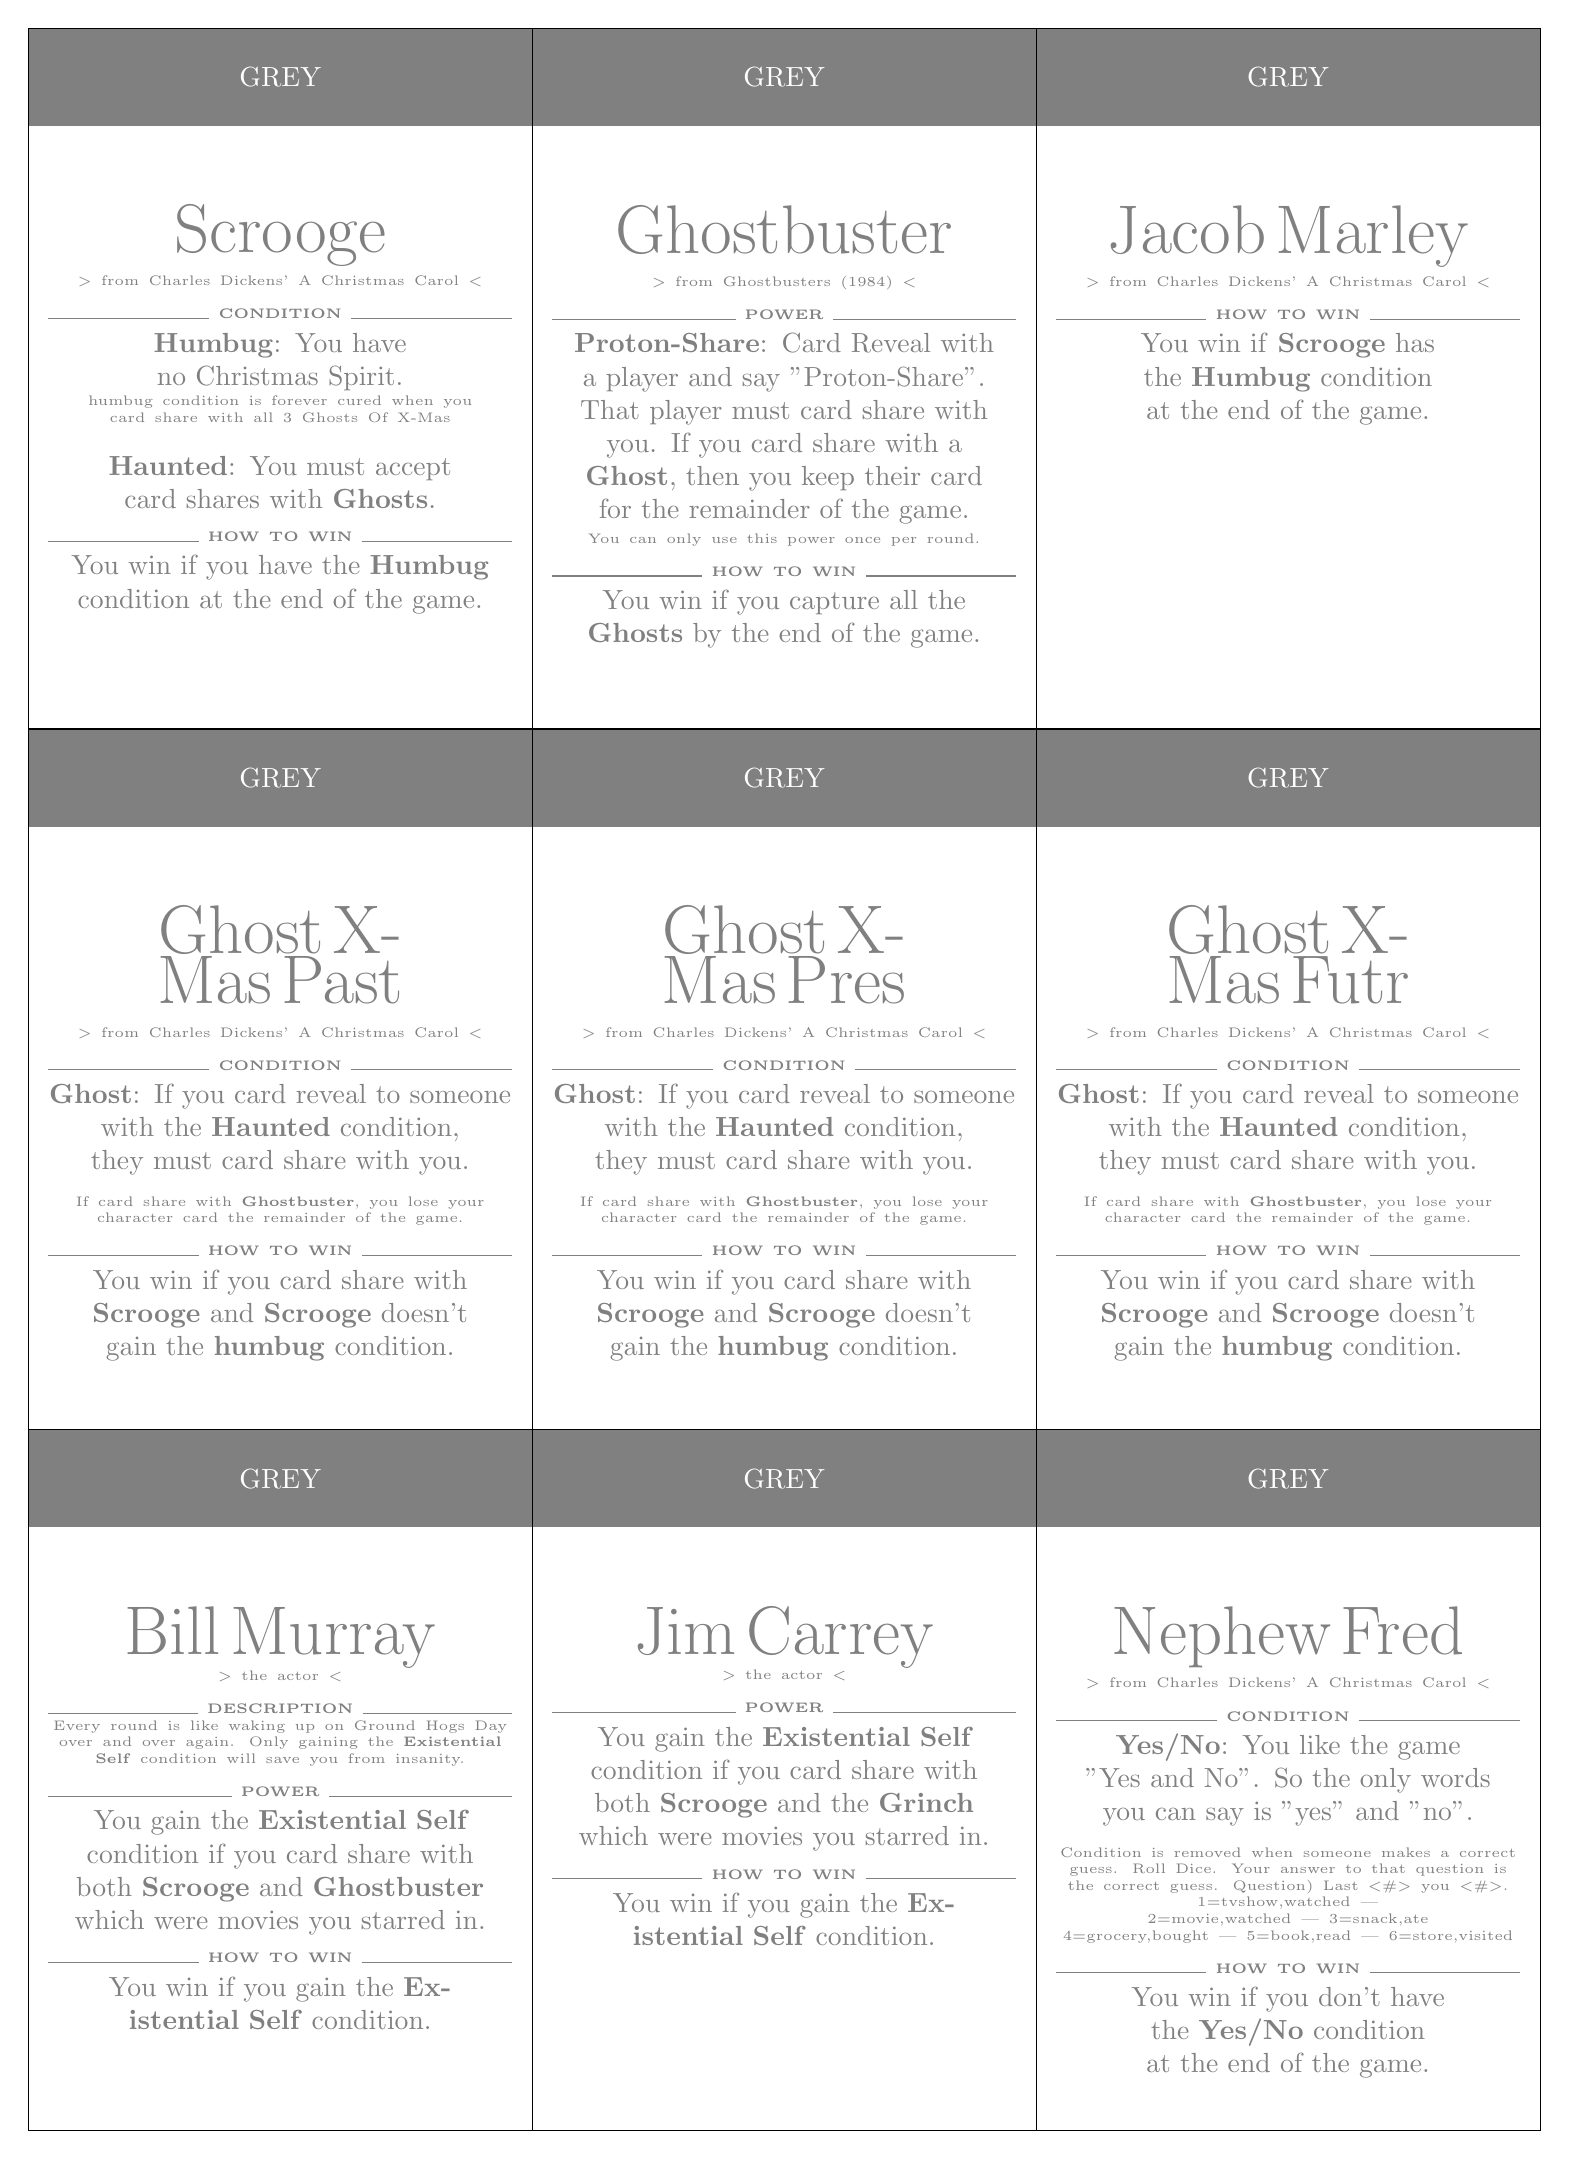
\begin{tikzpicture}[outer sep=0]
	
	% SCROOGE
	\node[teamshare, fill=gray] (1) at (3.2,26.7) {\HUGE GREY};
	\node[cardtext, text=gray] at (3.2,24.7) {
		{\Huge Scrooge}
		\titlefrom{Charles Dickens' A Christmas Carol}
		\seperatorcondition
		\condition{Humbug}: You have no Christmas Spirit.\\\vspace{0.05cm}
		\tiny humbug condition is forever cured when you card share with all 3 Ghosts Of X-Mas \\\vspace{0.25cm} \normalsize
		\condition{Haunted}: You must accept card shares with \character{Ghosts}.
		\seperatorwin
		You win if you have the \condition{Humbug} condition at the end of the game. \\
	};
	
	% GHOSTBUSTER
	\node[teamshare, fill=gray] at (9.6,26.7) {\HUGE GREY};
	\node[cardtext, text=gray] at (9.6,24.7) {
		{\Huge Ghostbuster}
		\titlefrom{Ghostbusters (1984)}
		\seperatoraction
		\condition{Proton-Share}: Card Reveal with a player and say "Proton-Share". That player must card share with you.
		If you card share with a \character{Ghost}, then you keep their card for the remainder of the game.
		\\\vspace{0.1cm}
		\tiny You can only use this power once per round. 
		\seperatorwin
		You win if you capture all the \condition{Ghosts} by the end of the game.
	};
	
	% JACOB MARLEY
	\node[teamshare, fill=gray] at (16,26.7) {\HUGE GREY};
	\node[cardtext, text=gray] at (16,24.7) {
		{\Huge Jacob Marley}
		\titlefrom{Charles Dickens' A Christmas Carol}
		\seperatorwin
		You win if \character{Scrooge} has the \condition{Humbug} condition at the end of the game.
	};
	
	% GHOST OF CHRISTMAS PAST
	\node[teamshare, fill=gray] at (3.2,17.8) {\HUGE GREY};
	\node[cardtext, text=gray] at (3.2,15.8) {
		{\Huge Ghost X-Mas Past}
		\titlefrom{Charles Dickens' A Christmas Carol}
		\seperatorcondition
		\condition{Ghost}: If you card reveal to someone with the \condition{Haunted} condition, they must card share with you.
		\\\vspace{0.25cm}
		\tiny If card share with \character{Ghostbuster}, you lose your character card the remainder of the game.
		\seperatorwin
		You win if you card share with \character{Scrooge} and \character{Scrooge} doesn't gain the \condition{humbug} condition.
	};
	
	% GHOST OF CHRISTMAS PRESENT
	\node[teamshare, fill=gray] at (9.6,17.8) {\HUGE GREY};
	\node[cardtext, text=gray] at (9.6,15.8) {
		{\Huge Ghost X-Mas Pres}
		\titlefrom{Charles Dickens' A Christmas Carol}
		\seperatorcondition
		\condition{Ghost}: If you card reveal to someone with the \condition{Haunted} condition, they must card share with you.
		\\\vspace{0.25cm}
		\tiny If card share with \character{Ghostbuster}, you lose your character card the remainder of the game.
		\seperatorwin
		You win if you card share with \character{Scrooge} and \character{Scrooge} doesn't gain the \condition{humbug} condition.
	};
	
	% GHOST OF CHRISTMAS FUTURE
	\node[teamshare, fill=gray] at (16,17.8) {\HUGE GREY};
	\node[cardtext, text=gray] at (16,15.8) {
		{\Huge Ghost X-Mas Futr}
		\titlefrom{Charles Dickens' A Christmas Carol}
		\seperatorcondition
		\condition{Ghost}: If you card reveal to someone with the \condition{Haunted} condition, they must card share with you.
		\\\vspace{0.25cm}
		\tiny If card share with \character{Ghostbuster}, you lose your character card the remainder of the game.
		\seperatorwin
		You win if you card share with \character{Scrooge} and \character{Scrooge} doesn't gain the \condition{humbug} condition.
	};
	
	% BILL MURRAY
	\node[teamshare, fill=gray] at (3.2,8.9) {\HUGE GREY};
	\node[cardtext, text=gray] at (3.2,6.9) {
		{\Huge Bill Murray}
		\\ \tiny > the actor <
		\seperatordescription
		\tiny Every round is like waking up on Ground Hogs Day over and over again. Only gaining the \condition{Existential Self} condition will save you from insanity.
		\seperatoraction
		You gain the \condition{Existential Self} condition if you card share with both \character{Scrooge} and \character{Ghostbuster} which were movies you starred in. 
		\seperatorwin
		You win if you gain the \condition{Existential Self} condition.
	};
	
	% JIM CARREY
	\node[teamshare, fill=gray] at (9.6,8.9) {\HUGE GREY};
	\node[cardtext, text=gray] at (9.6,6.9) {
		{\Huge Jim Carrey}
		\\ \tiny > the actor <
		\seperatoraction
		You gain the \condition{Existential Self} condition if you card share with both \character{Scrooge} and the \character{Grinch} which were movies you starred in.
		\seperatorwin
		You win if you gain the \condition{Existential Self} condition.
	};
	
	% NEPHEW FRED
	\node[teamshare, fill=gray] at (16,8.9) {\HUGE GREY};
	\node[cardtext, text=gray] at (16,6.9) {
		{\Huge Nephew Fred}
		\titlefrom{Charles Dickens' A Christmas Carol}
		\seperatorcondition
		\condition{Yes/No}: You like the game "Yes and No". So the only words you can say is "yes" and "no". \\\vspace{0.25cm}
		\tiny Condition is removed when someone makes a correct \\
		guess. Roll Dice. Your answer to that question is\\
		the correct guess. Question) Last <\#> you <\#>. \\
		1=tvshow,watched | 2=movie,watched | 3=snack,ate 
		\\4=grocery,bought | 5=book,read | 6=store,visited
		\seperatorwin
		You win if you don't have the \condition{Yes/No} condition at the end of the game.
	};
	
	
\draw (0,0) -- (19.2,0);
\draw (0,8.9) -- (19.2,8.9);
\draw (0,17.8) -- (19.2,17.8);
\draw (0,26.7) -- (19.2,26.7);

\draw (0,0) -- (0,26.7);
\draw (6.4,0) -- (6.4,26.7);
\draw (12.8,0) -- (12.8,26.7);
\draw (19.2,0) -- (19.2,26.7);
	
	
	
	\end{tikzpicture}
	
	%Background is not my own. But courtesy of a user on BGG
	
\includepdf[pages={1}, angle=90]{cardsbackground.pdf}
	
	
	
	
\end{document}